\section{Vorbetrachtung und Verwandte Arbeiten}
\label{sec:relatedwork}

Als erstes gilt es, gegenwärtige Technologien zu evaluieren, um eine solide Grundlage für eine verteilte Dateiverwaltung für die Schul-Cloud zu erstellen. Wie in der Einleitung erwähnt wurde, soll kein neuartiges Dateiverwaltungskonzept geschaffen werden. Vielmehr soll auf bestehenden Systemen und Technologien aufgebaut werden und deren Vorteile genutzt werden. Zu Beginn werden im Vorfeld formulierte Anforderungen aufgegriffen und analysiert. Hierzu diente der Technischen Bericht der Schul-Cloud \cite{paper:technischerbericht} als Grundlage, welcher in Zusammenarbeit des Hasso-Plattner-Instut mit dem Mint-EC enstand. Ebenfalls werden andere Konzepte zur Dateiverwaltung im Schul-Kontext durchsichtet und analysiert. Es schließt sich eine Beobachtung an, inwieweit Dateiablagen auf Basis von Cloud-Storage Providern bereits im Unterricht genutzt werden. Für eine abschließende Vorbetrachtung eignet sich eine Betrachtung bereits bestehender Cloud-Storage Anbieter, welche sich in der Praxis bewährt haben und weiträumigen Einsatz finden.

\subsection{Anforderungen an die Dateiverwaltung der Schul-Cloud}

\subsubsection{Die Cloud für Schulen in Deutschland: Konzept und Pilotierung der Schul-Cloud}

Der Technische Bericht der Schul-Cloud \cite{paper:technischerbericht} von (Meinel et. al) wurde von Wissenschaftlern am Hasso-Plattner-Institut in Potsdam geschrieben und beschäftigt sich mit einer ersten technischen Konzeption der Schul-Cloud. Dieser bildet die Grundlage für das Bachelor-Projekt der Schul-Cloud im Wintersemester 2016/17 und Sommersemester 2017, wessen sich diese Arbeit anschließt. Der Bericht beinhaltet im Kapitel 4.5 auch ein Konzept für das Dateimanagement. Dort wird beschrieben, dass Dateien auf allen Endgeräten verfügbar sein sollen. Außerdem wird ein Aufbau skizziert, auf den im weiteren Verlauf dieser Arbeit eingegangen wird (Kapitel 3). Weitere wichtige Aufgaben der Dateiverwaltung sollen das Speichern von ``zusätzlichen Metadaten, die Erzeugung von Thumbnails und die Verwaltung von Berechtigungen" \cite{paper:technischerbericht} sowie das Teilen von Inhalten sein.

\subsubsection{Studie „Bildung 2.0 - Digitale Medien in Schulen“}

Sinnbildlich für viele Studien im Bereich digitaler Bildung, zeigt dieser Bericht der BITKOM \cite{paper:studiebildung20} auf, dass die Bereitschaft von Schülern und Schülerinnen, von physischen zu digitalen Lerninhalten stetig wachse. Immer öfter diene ein Computer als Hilfe für die Bearbeitung von Hausaufgaben. Dies Zeigt auch die Abbildung \ref{fig:BitkomNutzungComputerStudie}. Auch kämen PCs öfter im Unterricht zum Einsatz. Allerdings würde die Qualität der IT-Infrastruktur nicht immer als positiv wahrgenommen. Der Wunsch nach besserer Ausstattung und intensiverem Nutzen von elektronischen Medien sei klar ersichtlich. Somit scheint eine Verbindung der Dateiverwaltung der Schul-Cloud mit dem Hausaufgaben - Dienst und Kursen sowie Fächern äußert sinnvoll, weshalb sich in dieser Arbeit vermehrt darauf bezogen wird.

\begin{figure}[H]
	\centering
	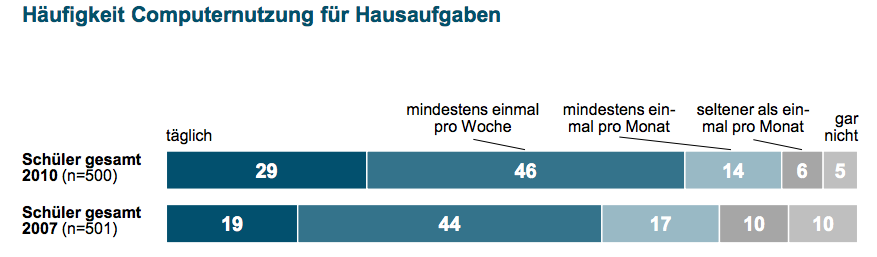
\includegraphics[width=0.8\linewidth]{images/BitkomNutzungComputerStudie}
	\caption[Caption for relatedWork]{Häufigkeit der Computernutzung für Hausaufgaben im Vergleich von 2007 zu 2010\footnotemark}
	\label{fig:BitkomNutzungComputerStudie}
\end{figure}
\footnotetext{Studie „Bildung 2.0 - Digitale Medien in Schulen“ (Folie 14) \cite{paper:studiebildung20}}

\subsubsection{Conceptual Architecture Design and Configuration of a Peer to Peer File System for Schools and Medium Sized Business}

Damian Clarke evaluierte in seinem Paper den Einsatz eines verteilten Dateisystem für Schulen und kleine Firmen \cite{paper:p2pfilesystemclarke}. Die Idee ist es, weg von einem üblichen zentralen Dateiserver zu einem verteilten Peer-to-Peer \footnote{Peer-to-Peer, eine gleichgestellte Rechner-zu-Rechner - Verbindung - \url{https://de.wikipedia.org/wiki/Peer-to-Peer}} zu wechseln, um so eine bessere Auslastung und ein skalierbares System zu erzielen. Gerade in der Schullandschaft sei es von Vorteil, auf eine verteilte Struktur zu setzen, da die Masse an Daten stetig zu nähme und die Kosten für Wartung und Erweiterung auf mehrere Träger besser zu verteilen wären. Dies ist besonders wichtig im Hinblick auf die Masse an Schulen in der Schul-Cloud. Wo zu Beginn noch 26 Partner-Schulen auf dem Produktivsystem unterwegs sind, werden dies mit Ausweitung nach der Pilotphase immer mehr. Somit macht eine Verteilung der Dateibestände auf mehrere Server Sinn.

\subsection{Nutzung von Cloud-Storage Providern im Unterricht}


Die Verwaltung von eigenen und geteilten Dateien wird mit der zunehmenden Digitalisierung des Unterrichts immer wichtiger. Wo es früher reichte, seine Unterrichtsmaterialien in einem Schulhefter zu legen, will man Arbeitsblätter und Wissenstexte heute überall und immer verfügbar haben. Um einen Eindruck in diese Problematik zu bekommen, wurde eine Umfrage zum Thema 'Dateiorganisation in der Schule' \cite{survey:umfragedateiorganisation} erstellt und an ehemaligen und aktuellen Schülern sowie Lehrern geschickt. Insgesamt nahmen \textbf{\textit{65}} \todo{Anpassen} Teilnehmer  an dieser Umfrage teil. Gefragt wurde unter anderem nach der Rolle des Teilnehmers (Schüler oder Lehrer) gefragt (Frage 1). Dabei sollten ehemalige Schüler und Lehrer vergangene Erfahrungen in die Beantwortung der Frage einfließen lassen. Dann wurde danach gefragt, ob der Befragte webbasierte Anwendungen zur Verwaltung der Dateien im Schulalltag benutzt hat (Frage 2). Anschließend wurde die Befragung geteilt. Wenn die Frage 2 mit 'Nein' beantwortet wurde, wurde nach Gründen für das Nichtbenutzen gefragt (Frage 3). Wurde Frage 2 mit 'Ja' beantwortet, wurde nach Vorteilen der Nutzung gefragt (Frage 4), sowie nach Beispielen, welche Dienste genutzt wurden (Frage 5). 

Die Ergebnisse \cite{survey:umfragedateiorganisationergebnisse} dieser Umfrage zeigen, dass eine Mehrheit der Befragten (ca. 72\%) auf solche Anbieter in ihrem Schulalltag verzichtet haben. Ein Großteil dieser Mehrheit gab an, dass Datenschutz ein großes Problem dabei darstellte. Ausländische Anbieter wie Dropbox \footnote{Dropbox - \url{https://www.dropbox.com/de/?landing=cntl}} oder Google Drive \footnote{Google Drive - \url{https://www.google.com/intl/de_ALL/drive/}} werden im pädagogischen Bereich eher kritisch betrachtet, da sie nicht in Deutschland gehostet werden und somit keine Transparenz in der Weiternutzung anfallender Daten erfolgt. Auch sind solche Dienste in Lernplattformen eher verpönt, da ``Schulen keinen Einfluss auf die Verwendung und Weiternutzung der hier anfallenden Daten und haben keine Vertragsbeziehung mit dem Betreiber dieser Dienste" \cite{online:itslearningmythenundfakten} haben. Weitere Gründe für die Nichtnutzung sind unter anderem, dass weite Teile des Unterrichtsmaterials offline zur Verfügung stehen, wie zum Beispiel einfache Arbeitsblätter, welche gar nicht erst digitalisiert werden. Oft ist auch einfach die Bereitschaft auf Seiten von Lehrer und Schüler gar nicht vorhanden, ihre Dateien online verfügbar zu machen, da die Ausstattung an den Schulen ohnehin auf einen weniger digitalen Unterricht ausgerichtet ist. Dazu kommen veraltete Technologien und schnelles Internet. Somit besteht auch kein Interesse daran, diese Dateien nur für den Gebrauch zu Hause verfügbar zu machen. Wenn dann doch Dateien von zu Hause in die Schule gebracht werden müssen, zum Beispiel Präsentationen oder Videos, wurden diese einfach auf einem USB-Stick gelagert.

Ein kleiner Teil der Befragten (ca. 28 \%) nutzten oder nutzen dagegen bereits Cloud-Storage Dienste für ihre Dateiverwaltung. Als meistgenutzter Dienst wurden hier Google Drive, One Drive  \footnote{One Drive - \url{https://onedrive.live.com/}} und Dropbox genannt. Ein sehr kleiner Teil benutzte sogar selbstgehostete Dienste wie zum Beispiel eine ownCloud \footnote{ownCloud - \url{https://owncloud.org/}}. Die Gründe hierfür seien die stetige Verfügbarkeit von mehreren Geräten, die papierlose Nutzung von Unterrichtsmaterialien, ein leichterer Backup von wichtigen Dateien und das Teilen mit mehren Personen. 

Die Auswertung der Umfrage zeigt, dass bei einem Großteil die Nutzung von cloudbasierten File-Storage Diensten eher auf Kritik stößt, als sie wirklich genutzt werden. Vor allem sind Datenschutz und schlechter Umgang mit digitalen Medien im Unterricht die Gründe hierfür. Mit einer einfachen Lösung innerhalb der Schul-Cloud, schnell an nötige Dateien für den Unterricht oder Hausaufgaben in digitaler Form zu kommen, könnte man hier ein Umdenken umleiten und die Vorteile sichtbar machen.

\subsection{Bestehende Cloud-Storage Provider}

Die Dateiverwaltung der Schul-Cloud soll nicht konzeptionell von Grund auf neu erstellt werden. Vielmehr soll auf bereits gut funktionierende und weit verbreitete Dienste zurückgegriffen werden. Auch soll es möglich sein, dass eine Schule selbst die Art des Hostings übernehmen kann, somit muss die Dateiverwaltung mehrere Typen einbinden können. Dies wird im Kapitel 3 als Form des Strategy-Patterns eingeführt, wodurch es möglich ist, Adapter für bestehende Anbieter zu schreiben. Im Folgenden werden solche Anbieter betrachtet, welche als erstes in die Schul-Cloud integriert wurden und werden sollen.

\subsubsection{AWS S3}

Als Teil der im Jahre 2006 eingeführten Amazon Web Services \footnote{Amazon Web Services - \url{https://aws.amazon.com/de/}} (AWS) bietet Amazon S3 (Simple Storage Service) als skalierbares Speichersystem zur Verfügung. S3 tritt hierbei als cloudbasierter Objektspeicher auf, der auf \textit{Buckets} und \textit{Objects} als Grundeinheiten basiert. Ein Bucket dient als einer Art Container, in dem mehrere Objects abgelegt werden. Ein Object ist somit eine Datei, die über einen \textit{Key} eindeutig in einem Bucket referenziert ist. In diesen Keys spiegelt sich auch die Ordnerstruktur innerhalb eines Bucket bzw. einen S3-Servers wieder. Dieser Aufbau wird als Quasi-Standard innerhalb von Storage Providern etabliert, wodurch sich die Dateiverwaltung der Schul-Cloud diesen Standard zu Nutze machen kann.

\subsubsection{ownCloud}

Die ownCloud ist eine Open Source Technologie zum Verwalten von Dateien. Sie wird oft dazu benutzt, um Dateien über mehrere Geräte synchronisieren. Für die Synchronisierung der Dateiablage greift ownCloud auf WebDAV zurück \footnote{Web-based Distributed Authoring and Versioning (WebDAV) - \url{https://de.wikipedia.org/wiki/WebDAV}}. Somit bring eine ownCloud den Vorteil mit sich, dass man darauf existierende Dateiablagen wie eine lokale Dateiverwaltung bearbeiten kann. Aufgrund des Open Source Status wird es oft als selbstgehostetes System an Schulen und Einrichtungen benutzt. Man erwartet sich hier maximalen Datenschutz, da keine Daten an kommerzielle Anbieter weitergereicht werden müssen. Dadurch ist die ownCloud ein interessantes Objekt für die Anbindung an die Schul-Cloud, da man selbst als Open Source Projekt auftritt.

\subsubsection{Dropbox}

Dropbox tritt seit 2007 als kommerzieller Filehosting-Dienst auf. Neben der Funktion als Cloud Storage Provider bietet es außerdem das Teilen von Dateien auf mehrere Nutzer. Ähnlich wie ownCloud hat man hier die Möglichkeit, über einen Sync-Client die in der Cloud abgespeicherten Dateien auf lokalen Rechnern zu bedienen. Die Umfrage aus Abschnitt 2.2., dass die Benutzung von kommerziellen Anbietern wie Dropbox kritisiert wird. Somit wird es keine direkte Dropbox-Anbindung in der Schul-Cloud geben. In Sachen Nutzerfreundlichkeit und Bedienbarkeit hat sich die Dateiverwaltung der Schul-Cloud jedoch ein Vorbild genommen. 

\clearpage
